\documentclass[11pt]{article}
\usepackage[a4paper,margin=23mm,headheight=14pt]{geometry}
\usepackage{fontspec,graphicx}
\usepackage{polyglossia}
\setmainlanguage{english}
\setotherlanguages{arabic,greek}
\setmainfont{Linux Libertine O}
\newfontfamily\arabicfont{Amiri}[Script=Arabic]
\newfontfamily\greekfont{FreeSerif}[Script=Greek]
\newfontfamily\syriacfont{Noto Sans Syriac}[Script=Syriac]
\usepackage{fancyhdr}
\usepackage[unicode,hidelinks]{hyperref}
\hypersetup{pdftitle={S01 v003 - Critical notes and source limitations},pdfauthor={Digital editorial apparatus; AI-assisted production}}
\graphicspath{{../source/presentation/}}
\pagestyle{fancy}\fancyhf{}\fancyhead[L]{S01 v003 — Critical notes}\fancyhead[R]{Modern editorial apparatus}\fancyfoot[C]{\thepage}
\setlength{\parindent}{0pt}\setlength{\parskip}{5pt}
\emergencystretch=2em
\begin{document}
\begin{center}{\Large Critical notes and source limitations}\par
{\large Nallino, Part I: front matter and apparatus}\par
S01 v003 — 25 September 2026\end{center}
These notes belong to the digital production, not to Nallino's historical prose. The historical reader is a separate artifact. Intrinsic quotations in Nallino retain their original languages; no new parallel translation has been generated.

The first-pass transcription covers the complete S01 range. This successor records a targeted reread of recovered proof material, not a new independently audited full transcription. Historical wording and errors remain distinguished from errors introduced by the digital transcription.

The ledger contains 85 successor decisions: 71 digital text repairs and 14 new image-fallback substitutions. Of the 14 critical entries, 3 now retain source-supported character readings, 10 preserve unresolved character distinctions through exact source images, and one records truncation already present in the frontispiece. Image preservation does not settle the interpretation of an uncertain character.

Source identifiers are physical pages of the pinned master, SRC01, not the reader's pagination. Every figure crop has a native-image rectangle and checksum. Nallino's own printed addenda are transcribed and routed, never silently applied to the earlier text.

\par\noindent\begin{minipage}{\linewidth}
\subsection*{S01-U001 — AB01-PDF0002}
\textit{source loss documented; reader p. 2}
The source panel is already cut at top/bottom and lateral edges. Cropping the provider bands cannot recover lost information.
\textbf{Reading.} surviving astronomical panel.
\textbf{Interpretive limit.} No reconstruction of the missing edges is proposed..
\textbf{Location.} {\small\texttt{AB01-PDF0002}}. review region.
\end{minipage}\par\smallskip
\par\noindent\begin{minipage}{\linewidth}
\subsection*{S01-U002 — AB01-PDF0018}
\textit{source reading retained; reader p. 9}
The native reread confirms the two unvocalized words \textarabic{المثبتة} and \textarabic{المبينة}. Retain the existing unvocalized transcription; no shaddah or other vowel mark is supplied.
\textbf{Reading.} \textarabic{المثبتة} / \textarabic{المبينة}.
\textbf{Location.} {\small\texttt{AB01-PDF0018-notes\_left-L024}}. whole source page; exact page anchor, not a fabricated line box.
\end{minipage}\par\smallskip
\par\noindent\begin{minipage}{\linewidth}
\subsection*{S01-U003 — AB01-PDF0022}
\textit{exact-image disposition; interpretation limited; reader p. 13}
The Syriac place-name is preserved in its existing exact image. Its Unicode transcription is not promoted.

\includegraphics[height=6mm]{AB01-PDF0022-G01.png}\hspace{4mm}
\par
\textbf{Interpretive limit.} Possible unvocalized bases \RL{{\syriacfont ܒܛܢ}} / \RL{{\syriacfont ܒܛܢܢ}}; vowel/diacritic encoding not resolved.
\textbf{Location.} {\small\texttt{AB01-PDF0022-body-L026}}. Individual crop coordinates and object hashes are recorded in the figure ledger.
\end{minipage}\par\smallskip
\par\noindent\begin{minipage}{\linewidth}
\subsection*{S01-U004 — AB01-PDF0040}
\textit{exact-image disposition; interpretation limited; reader p. 31}
The original Persian cluster includes more visible signs than the earlier \textarabic{زِگ} encoding represented. Replace that provisional encoding with the entire native cluster; do not guess a normalized Persian spelling.

\includegraphics[height=6mm]{AB01-PDF0040-G01.png}\hspace{4mm}
\par
\textbf{Interpretive limit.} \textarabic{زِگ} / \textarabic{زیگ}.
\textbf{Location.} {\small\texttt{AB01-PDF0040-notes\_left-L020}}. Individual crop coordinates and object hashes are recorded in the figure ledger.
\end{minipage}\par\smallskip
\par\noindent\begin{minipage}{\linewidth}
\subsection*{S01-U005 — AB01-PDF0040}
\textit{source reading retained; reader p. 31}
Native reread supports unaccented \textgreek{βιβλιον} in this quotation. Preserve that printed form, rather than adding the expected Greek accent.
\textbf{Reading.} \textgreek{βιβλιον}.
\textbf{Location.} {\small\texttt{AB01-PDF0040-notes\_right-L008}}. whole source page; exact page anchor, not a fabricated line box.
\end{minipage}\par\smallskip
\par\noindent\begin{minipage}{\linewidth}
\subsection*{S01-U006 — AB01-PDF0056}
\textit{source reading retained; reader p. 47}
The damaged initial letter is read as i in i. e.; comparison with the clean i. e. on the same mathematical page supports retaining the existing reading. Formula content is unchanged.
\textbf{Reading.} i. e..
\textbf{Location.} {\small\texttt{AB01-PDF0056-body-L020}}. whole source page; exact page anchor, not a fabricated line box.
\end{minipage}\par\smallskip
\par\noindent\begin{minipage}{\linewidth}
\subsection*{S01-U007 — AB01-PDF0070}
\textit{exact-image disposition; interpretation limited; reader p. 61}
Retain the existing exact sign image. Identification as alif with waslah remains an interpretation, not a substituted code point.

\includegraphics[height=6mm]{AB01-PDF0070-G01.png}\hspace{4mm}
\par
\textbf{Interpretive limit.} \textarabic{ٱ} (alif with waslah) is plausible; separate alif plus unidentified upper sign remains possible.
\textbf{Location.} {\small\texttt{AB01-PDF0070-body-L019}}. Individual crop coordinates and object hashes are recorded in the figure ledger.
\end{minipage}\par\smallskip
\par\noindent\begin{minipage}{\linewidth}
\subsection*{S01-U008 — AB01-PDF0070}
\textit{exact-image disposition; interpretation limited; reader p. 61}
Six unusually vocalized examples are now preserved as exact native clusters, including the two additional examples on the same lines. The placement of vowels and lower marks is no longer silently approximated by modern Unicode vowel sequences.

\includegraphics[height=6mm]{AB01-PDF0070-G02.png}\hspace{4mm}

\includegraphics[height=6mm]{AB01-PDF0070-G03.png}\hspace{4mm}

\includegraphics[height=6mm]{AB01-PDF0070-G04.png}\hspace{4mm}

\includegraphics[height=6mm]{AB01-PDF0070-G05.png}\hspace{4mm}

\includegraphics[height=6mm]{AB01-PDF0070-G06.png}\hspace{4mm}

\includegraphics[height=6mm]{AB01-PDF0070-G07.png}\hspace{4mm}
\par
\textbf{Interpretive limit.} Recorded consonants retained; precise vowel/sign attachment at these examples remains provisional.
\textbf{Location.} {\small\texttt{AB01-PDF0070-body-L021}}. Individual crop coordinates and object hashes are recorded in the figure ledger.
\end{minipage}\par\smallskip
\par\noindent\begin{minipage}{\linewidth}
\subsection*{S01-U009 — AB01-PDF0079}
\textit{exact-image disposition; interpretation limited; reader p. 70}
Preserve the original and corrected Arabic lemmas independently as exact images. Subbī/Ṣubbī remains typed. This records Nallino’s historical erratum; it does not apply the correction to printed p. XV.

\includegraphics[height=6mm]{AB01-PDF0079-G01.png}\hspace{4mm}

\includegraphics[height=6mm]{AB01-PDF0079-G02.png}\hspace{4mm}
\par
\textbf{Interpretive limit.} Latin consonant distinction confirmed; Arabic shaddah/vowel placements provisional.
\textbf{Location.} {\small\texttt{AB01-PDF0079-body-L021}}. Individual crop coordinates and object hashes are recorded in the figure ledger.
\end{minipage}\par\smallskip
\par\noindent\begin{minipage}{\linewidth}
\subsection*{S01-U010 — AB01-PDF0080}
\textit{exact-image disposition; interpretation limited; reader p. 71}
The left lemma visibly contains an intervening point or ink mark. It is now preserved as an image, so the two printed lemmas are no longer represented as visually identical words. Whether that point was intended is not decided.

\includegraphics[height=6mm]{AB01-PDF0080-G01.png}\hspace{4mm}
\par
\textbf{Interpretive limit.} The left lemma may be terrestri·um, with a small point or ink mark between i and u; the right is terrestrium. No different word ending is conjectured.
\textbf{Location.} {\small\texttt{AB01-PDF0080-body-L026}}. Individual crop coordinates and object hashes are recorded in the figure ledger.
\end{minipage}\par\smallskip
\par\noindent\begin{minipage}{\linewidth}
\subsection*{S01-U011 — AB01-PDF0082}
\textit{exact-image disposition; interpretation limited; reader p. 73}
Retain both existing exact lemma images, separately and in their original order. No character-level expansion is asserted.

\includegraphics[height=6mm]{AB01-PDF0082-G01.png}\hspace{4mm}

\includegraphics[height=6mm]{AB01-PDF0082-G02.png}\hspace{4mm}
\par
\textbf{Interpretive limit.} Tentative encodings \textarabic{واللول} / \textarabic{واللولوا} are withdrawn; alternative consonantal separation not promoted.
\textbf{Location.} {\small\texttt{AB01-PDF0082-body-L005}}. Individual crop coordinates and object hashes are recorded in the figure ledger.
\end{minipage}\par\smallskip
\par\noindent\begin{minipage}{\linewidth}
\subsection*{S01-U012 — AB01-PDF0084}
\textit{exact-image disposition; interpretation limited; reader p. 75}
Replace the uncertain fully vocalized transcription with two full native verse-line objects. Each preserves its original right-hand first hemistich and left-hand second hemistich. Earlier proposed text is retained only in version history and the change ledger, not certified as the reading.
\par\begin{center}
\includegraphics[width=.80\linewidth]{AB01-PDF0084-G01.png}\end{center}
\par\begin{center}
\includegraphics[width=.80\linewidth]{AB01-PDF0084-G02.png}\end{center}
\par
\textbf{Interpretive limit.} Consonantal verse retained; vowel placements in \textarabic{تُمِرُّ} / \textarabic{تَدُلَّ} and final case-vowels remain provisional.
\textbf{Location.} {\small\texttt{AB01-PDF0084-body-L028}}. Individual crop coordinates and object hashes are recorded in the figure ledger.
\end{minipage}\par\smallskip
\par\noindent\begin{minipage}{\linewidth}
\subsection*{S01-U013 — AB01-PDF0037}
\textit{exact-image disposition; interpretation limited; reader p. 28}
The source terminal digit in the first page number has a broken stroke. Exact pixels replace a confidently encoded 100; neither a numerical correction nor a conjecture is applied.
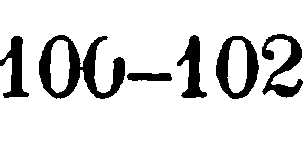
\includegraphics[height=6mm]{AB01-PDF0037-G01.png}\hspace{4mm}
\par
\textbf{Interpretive limit.} 100–102 / 106–102; the terminal digit is damaged.
\textbf{Location.} {\small\texttt{AB01-PDF0037-body-L017}}. Individual crop coordinates and object hashes are recorded in the figure ledger.
\end{minipage}\par\smallskip
\par\noindent\begin{minipage}{\linewidth}
\subsection*{S01-U014 — AB01-PDF0086}
\textit{exact-image disposition; interpretation limited; reader p. 77}
The printed title word is difficult to encode faithfully at the damaged medial letter. Preserve the exact source word rather than regularizing the Latin title.

\includegraphics[height=6mm]{AB01-PDF0086-G01.png}\hspace{4mm}
\par
\textbf{Interpretive limit.} precipua / previpua; the medial printed letter is unclear.
\textbf{Location.} {\small\texttt{AB01-PDF0086-body-L013}}. Individual crop coordinates and object hashes are recorded in the figure ledger.
\end{minipage}\par\smallskip
\section*{Version history, preservation and audit status}
The v002 release is preserved unchanged. All 535 files recorded in its self-excluding manifest matched their saved hashes. The interrupted reread left 157 recoverable proof images, but no revised transcription or decision ledger was found with them. Those images are preserved as recovery evidence; their headings were not accepted as reading authority.

The current producing assistant visually reread 562 general proof candidates and 164 targeted candidates. The counts refer to candidate snippets, with possible overlap, not 726 separate pages or an independent word-by-word audit. Confirmed differences were recorded as before/after decisions. Dense mathematical pages and the other formula-bearing source regions were also reread. No mathematical recalculation was used to overwrite the historical text.

The 86 historical addenda/corrigenda entries remain \texttt{REGISTERED\_NOT\_APPLIED}. Future-session anchors are routing references only. S02 has not begun. The Arabic authorial canon has not been altered.

The included rebuild program performs two clean two-pass builds and records their hashes. The read-only technical audit verifies file identity, coverage, exact native crop pixels, anchor consistency and build receipts. These are technical tests, not independent philological certification. The producing assistant is responsible for this reread and the changes; a separate cold source/reading auditor has not replayed this successor. S01 therefore remains open at that release gate.

Line-alignment rectangles inherited from embedded-text similarity are locator candidates, not independently certified measurements of every source line. Native image-crop coordinates have a separate pixel-equality check. Precise uncertainties are disclosed, rather than supplied from expected spelling, grammar or numerical coherence.

\section*{Source citation}
Nallino, C. A. (1903). [Front matter, preface, bibliography, and addenda]. In \textit{Al-Battānī sive Albatenii opus astronomicum} (Pars prima: \textit{Versio capitum cum animadversionibus}, pp. VII–LXXX). Ulrich Hoepli. Controlling digital witness: SRC01, physical PDF2, PDF10 and PDF12–89.

{\small Source SHA-256:\par\texttt{544c16b6355c9b74e281aded657d6572}\par\texttt{24bff738366d5260e1a610d31b0d6297}\par}
\end{document}
